\section{Anhang}


\subsection{Massenträgheitsmomente} %TODO: weiter vorne verpflanzen
\label{Massenträgheitsmomente}

\begin{center}
\begin{tabular}{| c | c |}
\hline
\textbf{Zylinder / Scheibe} & \textbf{Hohlzylinder} \\
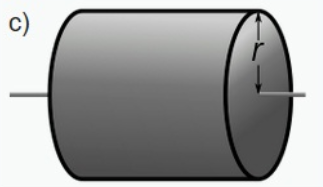
\includegraphics[width=0.35\linewidth]{Bilder/Wellen-Optik/J_zylinder} & 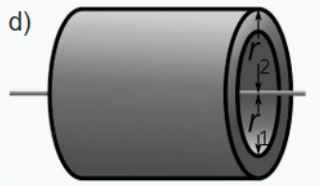
\includegraphics[width=0.35\linewidth]{Bilder/Wellen-Optik/J_hohlzylinder} \\
$J = \frac{1}{2} m r^2$ & $J = m \, \frac{r_1^2 + r_2^2}{2}$ \\
\hline
\textbf{Dünner Stab (Mitte)} & \textbf{Dünner Stab (Ende)} \\
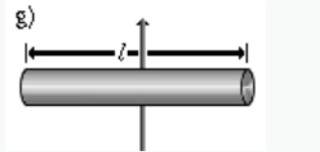
\includegraphics[width=0.35\linewidth]{Bilder/Wellen-Optik/J_duenner_stab_mitte} & 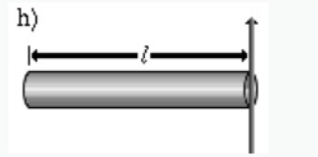
\includegraphics[width=0.35\linewidth]{Bilder/Wellen-Optik/J_duenner_stab_ende} \\
$J = \frac{1}{12} m l^2$ & $J = \frac{1}{3} m l^2$ \\
\hline
\textbf{Kugel} & \textbf{Massenpunkt} \\
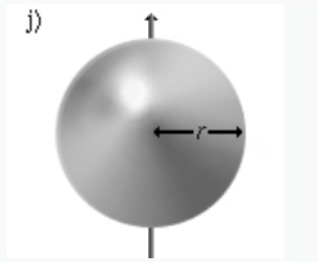
\includegraphics[width=0.35\linewidth]{Bilder/Wellen-Optik/J_kugel} & 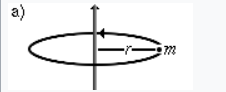
\includegraphics[width=0.35\linewidth]{Bilder/Wellen-Optik/J_massepunkt} \\
$J = \frac{2}{5} m r^2$ & $J = m r^2$ \\
\hline
\end{tabular}
\end{center}


\subsection{Messunsicherheit}

Abhängigkeit der Messgrösse: $ y = y(x_1,x_2,...,x_n) $

Unsicherheit der Messgrösse: \( \Delta y = \sqrt{\sum_{i} \left( \frac{\partial y}{\partial x_i}\right)^2 \Delta x_i^2} \)

Beispiel: $ f = \frac{c}{\lambda} $

\begin{align*}
	\Delta f &= \sqrt{\left( \frac{\partial f}{\partial c}\right)^2 \Delta c^2 + \left( \frac{\partial f}{\partial \lambda}\right)^2 \Delta \lambda^2} \\
	         &= \sqrt{\left( \frac{1}{\lambda}\right)^2 \Delta c^2 + \left( - \frac{c}{\lambda^2}\right)^2 \Delta \lambda^2} 
\end{align*}



\subsection{Trigonometrie}
		
		
		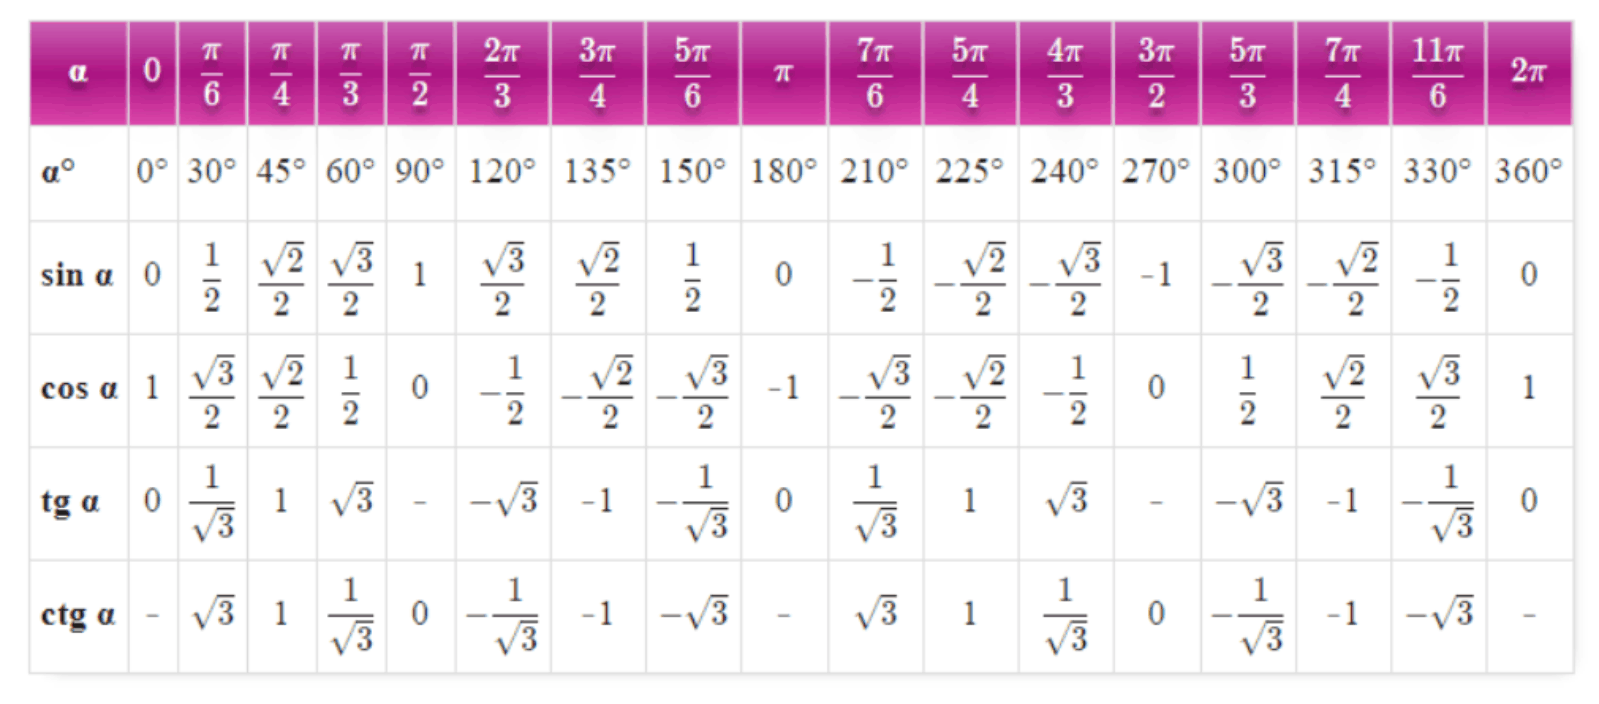
\includegraphics[width=\linewidth]{Bilder/Wellen-Optik/trigo} 
		
		\subsubsection{Beziehungen zwischen $\sin(x)$ und $\cos(x)$}
		\begin{tabular}{ll}
		$\sin(-a) = -\sin(a)$ & $\cos(-a) = \cos(a)$ \\
		$\sin(\pi - a) = \sin(a)$ & $\cos(\pi -a) = - \cos(a)$ \\		
		$\sin(\pi + a) = -\sin(a)$ & $\cos(\pi + a) = - \cos(a)$ \\	
		$\sin(\frac{\pi}{2} - a) = \sin(\frac{\pi}{2} + a) = \cos(a)$ \\
		$\cos(\frac{\pi}{2} - a) = - \cos(\frac{\pi}{2} + a) = \sin(a)$\\		 
		\end{tabular}
		
		
		% \vfill\null
		% \columnbreak

		\subsubsection{Additionstheoreme}
		
		$\sin(a \pm b) = \sin(a) \cdot \cos(b) \pm \cos(a) \cdot \sin(b)$ \\
		$\cos(a \pm b) = \cos(a) \cdot \cos(b) \mp \sin(a) \cdot \sin(b) $ \\
		$\tan(a \pm b) = \frac{\tan(a) \pm \tan(b)}{1 \mp \tan(a) \cdot \tan(b)}$
		
	
		\subsubsection{Summen und Differenzen}
		
		$\sin(a) + \sin(b) = 2 \cdot \sin \big( \frac{a+b}{2} \big) \cdot \cos \big( \frac{a-b}{2} \big)$ \\
		$\sin(a) - \sin(b) = 2 \cdot \sin \big( \frac{a-b}{2} \big) \cdot \cos \big( \frac{a+b}{2} \big)$ \\
		$\cos(a) + \cos(b) = 2 \cdot \cos \big( \frac{a+b}{2} \big) \cdot \cos \big( \frac{a-b}{2} \big)$ \\
		$\cos(a) - \cos(b) = -2 \cdot \sin \big( \frac{a+b}{2} \big) \cdot \sin \big( \frac{a-b}{2} \big)$ \\
		$\tan(a) \pm \tan(b) = \frac{\sin(a \pm b)}{\cos(a) \cdot \cos(b)}$ 
		
			
		
		\subsubsection{Produkte}
		$\sin(a) \cdot \sin(b) = \frac{1}{2} \big( \cos(a-b) - \cos(a+b) \big) $ \\
		$\cos(a) \cdot \cos(b) = \frac{1}{2} \big( \cos(a-b) + \cos(a+b) \big) $ \\	
		$\sin(a) \cdot \cos(b) = \frac{1}{2} \big( \sin(a-b) + \sin(a+b) \big) $ 
			
			
		\subsubsection{Winkelvielfache und Halbwinkel}
		$\sin(2a) = 2 \, \sin(a) \cdot \cos(a)$ \\
		$\sin(3a) = 3 \, \sin(a) -4 \, \sin^3(a)$ \\ 
		$\sin(4a) = 8 \, \cos^3(a) \cdot \sin(a) - 4 \, \cos(a) \cdot \sin(a)$ \\
		\vspace{0.2cm}
		$\cos(2a) = \cos^2(a) - \sin^2(a)$ \\
		$\cos(3a) = 4 \, \cos^3(a) -3 \, \cos(a)$ \\ 
		$\cos(4a) = 8 \, \cos^4(a) - 8 \, \cos^2(a) + 1$ \\
		\vspace{0.2cm}
		$\sin \big( \frac{a}{2} \big) = \sqrt{\frac{1}{2}(1-\cos(a))} $ \qquad $\cos \big( \frac{a}{2} \big) = \sqrt{\frac{1}{2}(1+\cos(a))} $ 
		
		
		\subsubsection{Potenzen}
		$\sin^2(a) = \frac{1}{2}(1-\cos(2a))$ \\	
		$\sin^3(a) = \frac{1}{4}(3\, \sin(a) - \sin(3a))$ \\	
		$\sin^4(a) = \frac{1}{8}(\cos(4a) -4 \, \cos(2a) +3)$ \\	
		\vspace{0.2cm}
		$\cos^2(a) = \frac{1}{2}(1+\cos(2a))$ \\	
		$\cos^3(a) = \frac{1}{4}(\cos(3a) + 3 \, \cos(a)$ \\	
		$\cos^4(a) = \frac{1}{8}(\cos(4a) +4 \, \cos(2a) +3)$ 